\documentclass[../TDON2_inter.tex]{subfiles}%

\begin{document}
\section[s]"1"{Trombone de \textsc{Kœnig}}

\enonce{%
	\noindent
	\begin{minipage}{0.70\linewidth}
		Le trombone de \textsc{Kœnig} est un dispositif de laboratoire permettant de
		faire interférer deux ondes sonores ayant suivi des chemins différents. Le
		haut-parleur, alimenté par un générateur de basses fréquences, émet un son
		de fréquence $f = \SI{1500\pm1}{Hz}$. On mesure le signal à la sortie avec
		un microphone branché sur un oscilloscope.
	\end{minipage}
	\hfill
	\begin{minipage}{0.30\linewidth}
		\begin{center}
			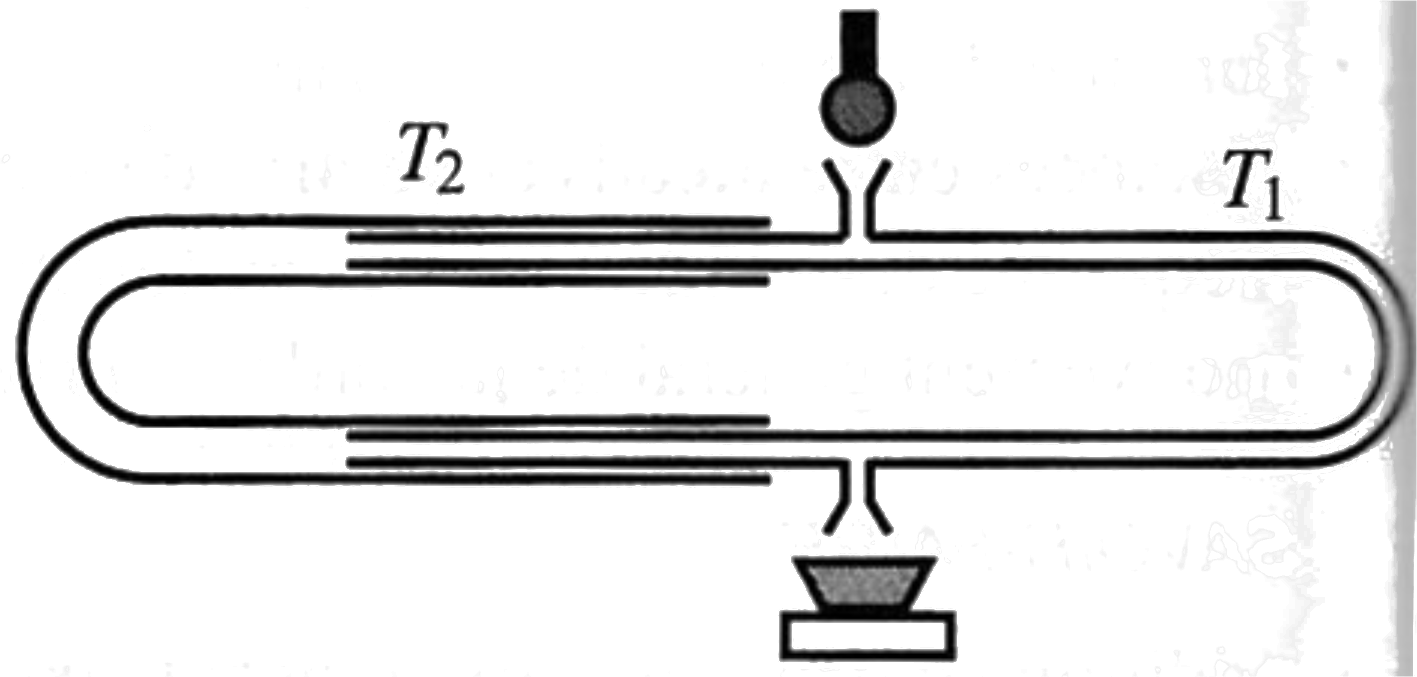
\includegraphics[width=\linewidth]{keonig-plain_white}
		\end{center}
	\end{minipage}
}

\QR{%
	Exprimer en fonction de la distance $d$ de coulissage de $T_2$ par
	rapport à $T_1$ le déphasage au niveau de la sortie entre l'onde sonore
	passée par $T_2$ et celle passée par $T_1$.
}{%
	\begin{gather*}
		\D\f_{2/1}(\Mr) = -k\D L_{2/1}(\Mr) = -k(\rm OT_2 - OT_1)
	\end{gather*}
	Or, si on déplace $T_2$ par rapport à $T_1$ de $d$, l'onde passant dans
	$T_2$ doit parcourir $2d$ de plus, une fois pour chaque partie
	rectiligne~; ainsi
	\[\boxed{\D\f_{2/1}(\Mr) = -2kd}\]
}

\QR{%
	En déplaçant la partie mobile $T_2$, on fait varier l'amplitude du
	signal observé. On observe que lorsqu'on déplace $T_2$ de $d =
		\SI{11.5\pm0.2}{cm}$, on passe d'un minimum d'amplitude à un autre. En
	déduire la valeur de la célérité du son dans l'air à
	\SI{20}{\degreeCelsius}, température à laquelle l'expérience est faite.
}{%
	Cette observation traduit qu'un décalage de \SI{11.5}{cm} fait passer
	d'une interférence destructive à celle qui la suit, donc augmente le
	déphasage de $2\pi$ ou la différence de marche de $\lambda$. On a donc
	\begin{gather*}
		\abs{\bcancel{2}kd} = \bcancel{2}\pi
		\Lra
		\frac{2\cancel{\pi}}{\lambda}d = \cancel{\pi}
		\Lra
		\boxed{2df = c}
		\qavec
		\left\{
		\begin{array}{rcl}
			d & = & \SI{11.5e-2}{m} \\
			f & = & \SI{1500}{Hz}
		\end{array}
		\right.\\
		\mathrm{A.N.~:}\quad
		\boxed{c = \SI{345}{m.s^{-1}}}
	\end{gather*}
}
\end{document}
